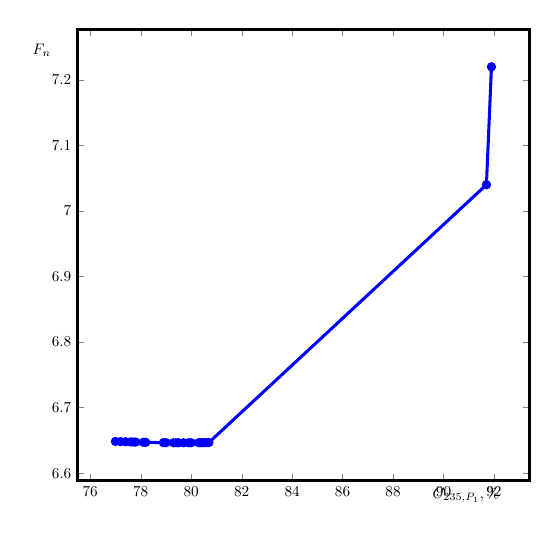
\begin{tikzpicture}[,
scale=0.55]
\begin{axis}[
  xlabel style = {{at={(axis description cs:.86,0)}}},
  ylabel = {$F_n$},
  ylabel style = {{at={(axis description cs:-0.08,.925)},rotate=270,anchor=south}},
  xlabel = {$C_{235,P_1}, \%$},
  width=12cm, height=12cm, line width=2pt
]

\addplot+ coordinates {
  (77.0, 6.648369301601674)
  (77.2, 6.6481081422427755)
  (77.4, 6.6478609680670795)
  (77.60000000000001, 6.647628620667707)
  (77.7, 6.647518634806713)
  (77.8, 6.647412135764082)
  (78.10000000000001, 6.647118512130983)
  (78.2, 6.64702925961305)
  (78.9, 6.6465428786148735)
  (79.0, 6.646493966987278)
  (79.3, 6.646383406485429)
  (79.4, 6.646358460860561)
  (79.5, 6.646339791250357)
  (79.7, 6.646321811441468)
  (79.9, 6.646330897249658)
  (80.0, 6.646346113745254)
  (80.30000000000001, 6.64643598238657)
  (80.4, 6.646481376154359)
  (80.5, 6.646534553797508)
  (80.60000000000001, 6.646596419821)
  (80.7, 6.646666619197229)
  (91.7, 7.040023902346512)
  (91.9, 7.219931649864452)
};

\end{axis}
\end{tikzpicture}

